\documentclass[tikz]{standalone}
\usetikzlibrary{automata,positioning}
\begin{document}
  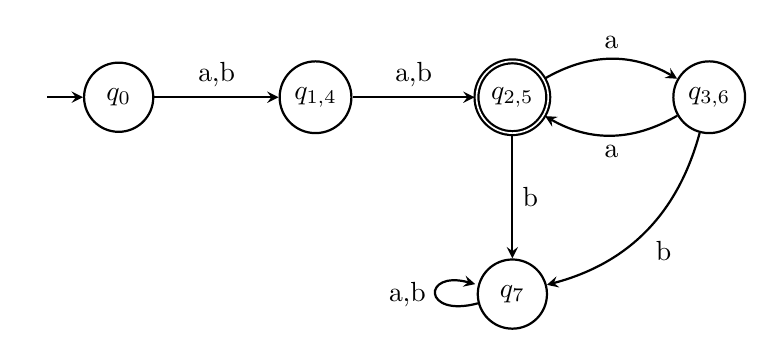
\begin{tikzpicture}[>=stealth,node distance=25mm,on grid,auto, thick, initial text=]
    \node[state,initial] (q0) {$q_0$};
    \node[state] (q14) [right=of q0] {$q_{1,4}$};
    \node[state, accepting] (q25) [right=of q14] {$q_{2,5}$};
    \node[state] (q36) [right= of q25] {$q_{3,6}$};
    \node[state] (q7) [below=of q25] {$q_7$};
    
    \path[->]
    (q0) edge node {a,b} (q14)
    (q14) edge node {a,b} (q25)
    (q25) edge [bend left] node {a} (q36)
    (q36) edge [bend left] node {a} (q25)
    (q25) edge node {b} (q7)
    (q36) edge [bend left] node {b} (q7)
    (q7) edge [loop left] node {a,b} (q7);
  \end{tikzpicture}

\end{document}